\documentclass[11pt,a4paper]{article}
\usepackage{cite}
\usepackage{apalike}
\usepackage{amsmath}
\usepackage{amsfonts}
\usepackage{amssymb}
\usepackage{makeidx}
\usepackage{graphicx}
\usepackage{wrapfig}
\usepackage{enumerate}
\usepackage{pdfpages}
\usepackage{tocloft}
\usepackage{setspace}
\usepackage{mathtools}
\usepackage{hyperref}
\definecolor{linkcolour}{rgb}{0,0.2,0.6} % Link color
\hypersetup{colorlinks,breaklinks,urlcolor=linkcolour,linkcolor=linkcolour, citecolor=linkcolour}

\usepackage[left=2cm,right=2cm,top=2cm,bottom=2cm]{geometry}

\usepackage{xcolor}

\usepackage{fontspec}
\setmainfont{Cambria}

\usepackage{caption}
\captionsetup[figure]{font=small, labelfont={bf}}
\captionsetup[table]{font=small, labelfont={bf}}

\usepackage{float}
\usepackage{multirow}
\usepackage{longtable}

\usepackage[nottoc]{tocbibind}

\setcounter{tocdepth}{4}
\setcounter{secnumdepth}{4}

\newcommand{\spa}{\vspace{1.25em}}
\newcommand{\noi}{\noindent}
\def\dul#1{\underline{\underline{#1}}}
\def\cpt#1#2{{\begin{center}\small\textbf{\textcolor{blue}{Figure #1:}} #2\end{center}}}

% for dots in the content
\usepackage{tocloft}
\renewcommand{\cftsecleader}{\cftdotfill{\cftdotsep}}

\begin{document}
	\begin{titlepage} 
		\begin{center}
		\large{MINI PROJECT 1}\\
		% \vspace{1em}
		\large {COGS 209 Scientific Data Analysis and Statistical Learning}
		\vspace{3em}
		
		\rule{0.9\linewidth}{0.5mm} \\[0.4cm]
	    {\Large{\bfseries{Depression Identification using Continuous Motor Activity}}} \\
	    \rule{0.9\linewidth}{0.5mm} \\[3 em]	
	    
	    \vspace{5em}

	    Lead Author: Sowmya Manojna Narasimha\\

	    \vspace{1em}

	    Co-Authors: Morgan Fitzgerald, Michaela Cullum-Doyle, Vanessa Martin\\

		\vspace{25em}

		University of California, San Diego
		
		\vspace{5em}    
	    
    	% \includegraphics[scale = 0.09]{images/iitmlogo.png}
		\end{center}
	\end{titlepage}

{\hypersetup{linkcolor=black}
 \tableofcontents}
\break

\section{Introduction}
\subsection{Background}
The global incidence of depression is on the rise \cite{marrie2019rising}. This alarming trend highlights the urgent need for new and effective tools to detect and treat depression. Early detection and treatment of depression are crucial for improving outcomes and preventing further complications. Fortunately, recent advancements in technology have opened up new avenues for detecting and tracking depression using digital tools. One promising idea is to use motor activity data to classify the depressive state of individuals \cite{aminifar2021monitoring}, \cite{garcia2018depresjon}. This approach is exciting as it has the potential to overcome the limitations of canonical depressive-symptom surveys and provide a more objective measure of an individual's depressive state.\\

\noi
In this study, we aim to investigate the potential of motor activity as a predictor of depressive states using motor activity (actigraph data) from \cite{garcia2018depresjon}. We will leverage several classifications models including Logistic Regression, Random Forests, K-Nearest Neighbors, Support Vector Machines, and Multi-Layered Perceptrons, and compare their performance in predicting depression based on motor activity. We will include sex and age as covariates in our analysis, as they may impact motor activity and have implications for the accuracy of our models. We hypothesize that the random forest algorithm will outperform the linear regression model in classifying depressive state based on motor activity data (H1). We also expect that age and sex will have a significant impact on motor activity and that including them as covariates in the logistic regression model will improve its performance in depression classification (H2). Finally, we predict that the model will perform better on males compared to females due to potential differences in motor activity patterns between sexes (H3) and on individuals with severe depression compared to mild/moderate depression as their motor activity may be more significantly impacted by their depressive state (H4). Overall, this study has important implications for the development of accurate and reliable tools for detecting and tracking depression using machine learning algorithms and digital tools.

\section{Methods}
\subsection{Data}
\subsubsection{Description}
For all of our analysis, we used the \textit{Depresjon} dataset presented in \cite{garcia2018depresjon}. The dataset consists of movement activity, actigraph data data recorded using a wrist watch (actiwatch). The actiwatch measures activity as a function of the duration, amount and intensity of movement in all directions, using a piezo-electric accelerometer. The total activity count was measured in 1 minute periods.\\

\noi
The actigraph data was measured from 23 patients who were diagnosed with depression and 32 control subjects. In addition to the actigraph data from each of the participants, meta data about each participant was also made available. The fields present in the meta data are as follows:
\begin{enumerate}
	\itemsep0em
	\item \texttt{number}: Patient Identifier (Control or Condition)
	\item \texttt{days}: Number of days of measurements
	\item \texttt{gender}: Gender indicator (1: Females, 2: Males)
	\item \texttt{age}: Age in age groups
	\item \texttt{afftype}: Type of depression (1: Bipolar Depression II, 2: Unipolar Depression, 3" Bipolar 
	Depression I)
	\item \texttt{melanch}: Melancholia Identifier (1: Melancholia, 2: No melancholia)
	\item \texttt{inpatient}: Inpatient Identifier (1: Inpatient, 2: Outpatient)
	\item \texttt{edu}: Education-level grouped in years
	\item \texttt{marriage}: Marriage/Relationship Indicator (1: Married/Cohabiting, 2: Single)
	\item \texttt{work}: Work Indicator: (1: Working/Studying, 2: Unemployed/On a Sick Leave/Receiving Pension)
	\item \texttt{madrs1}: MADRS score when measurement started
	\item \texttt{madrs2}: MADRS score when measurement stopped
\end{enumerate}

\subsubsection{Preprocessing}
\paragraph{Meta Data Imputation}
The meta data provided with the actigraph data, had missing entries. The missing value imputations were performed using a K-Nearest Neighbors based imputation. The neighbors were weighted based on their distance for the imputation and points that were closer were given higher weightage. 

% The visualization of the same is as follows:

% \begin{figure}[H]
% 	\centering
% 	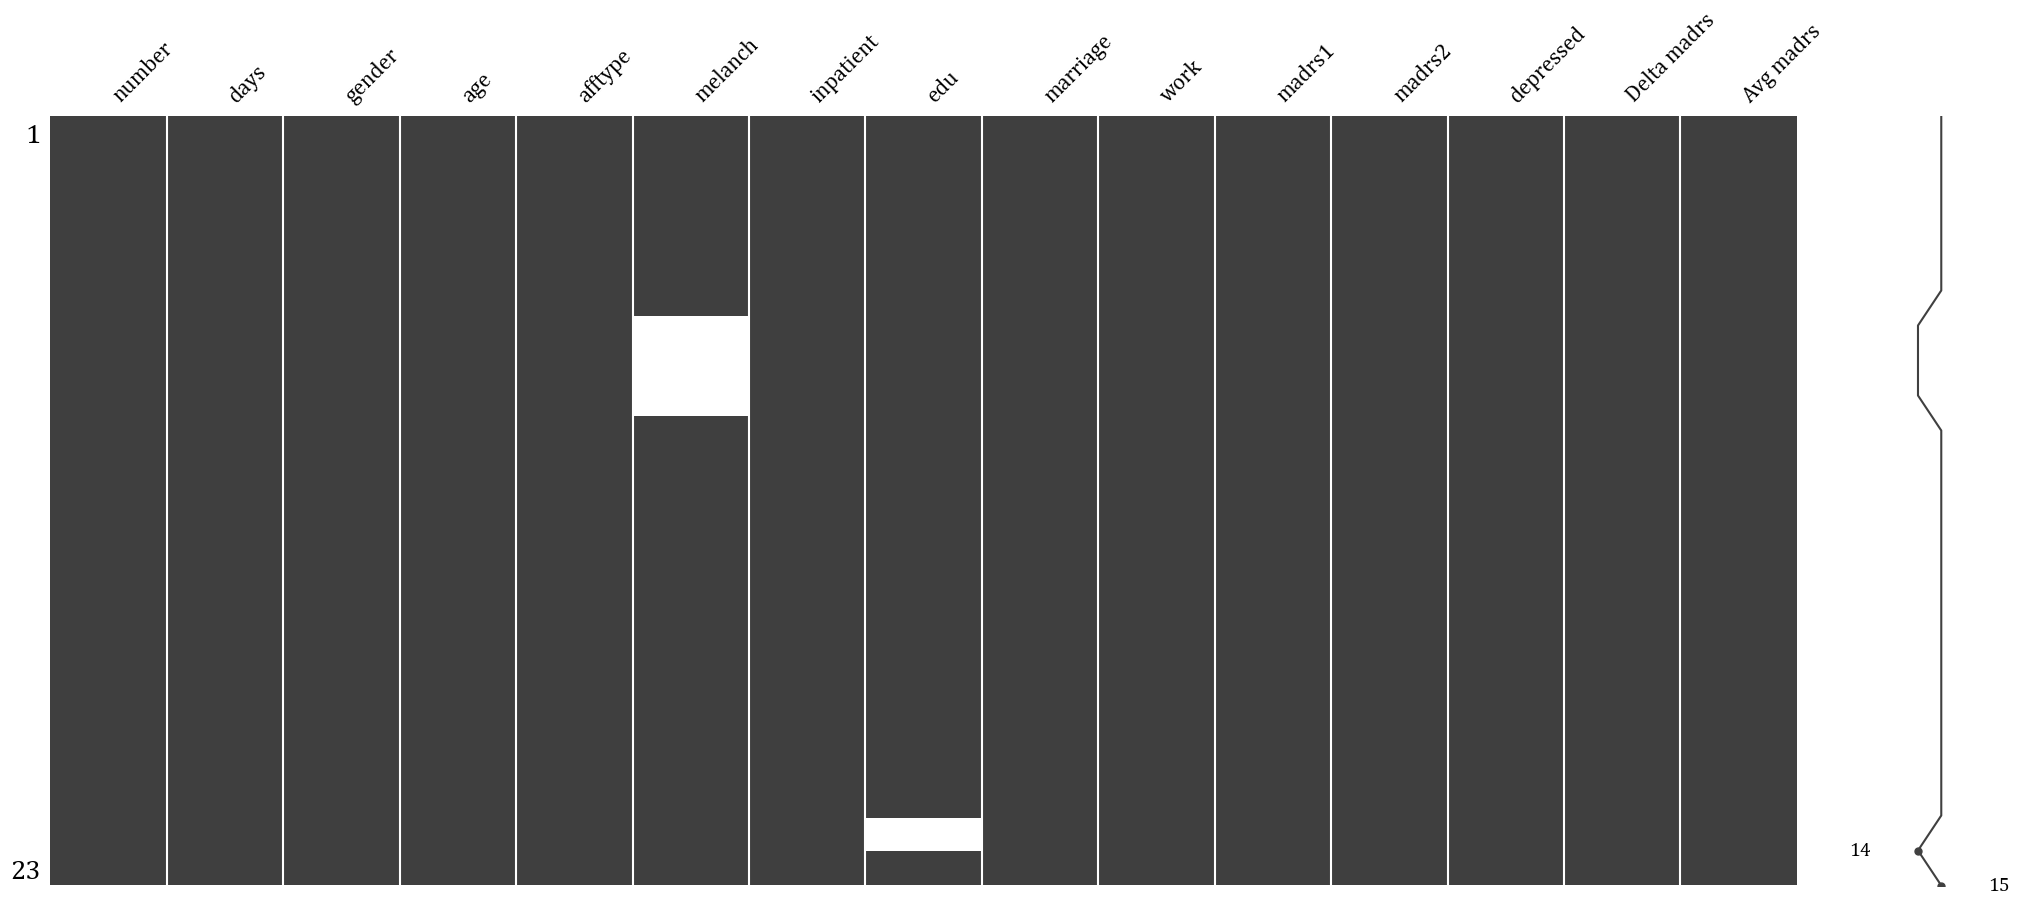
\includegraphics[scale=0.3]{images/missingno_init.png}
% 	\caption{Visualization of missing values in the meta data. White horizontal bars indicate missing values.}
% 	\label{fig:missing_init}
% \end{figure}
% The visualization of the data after imputation is as follows:
% 
% \begin{figure}[H]
% 	\centering
% 	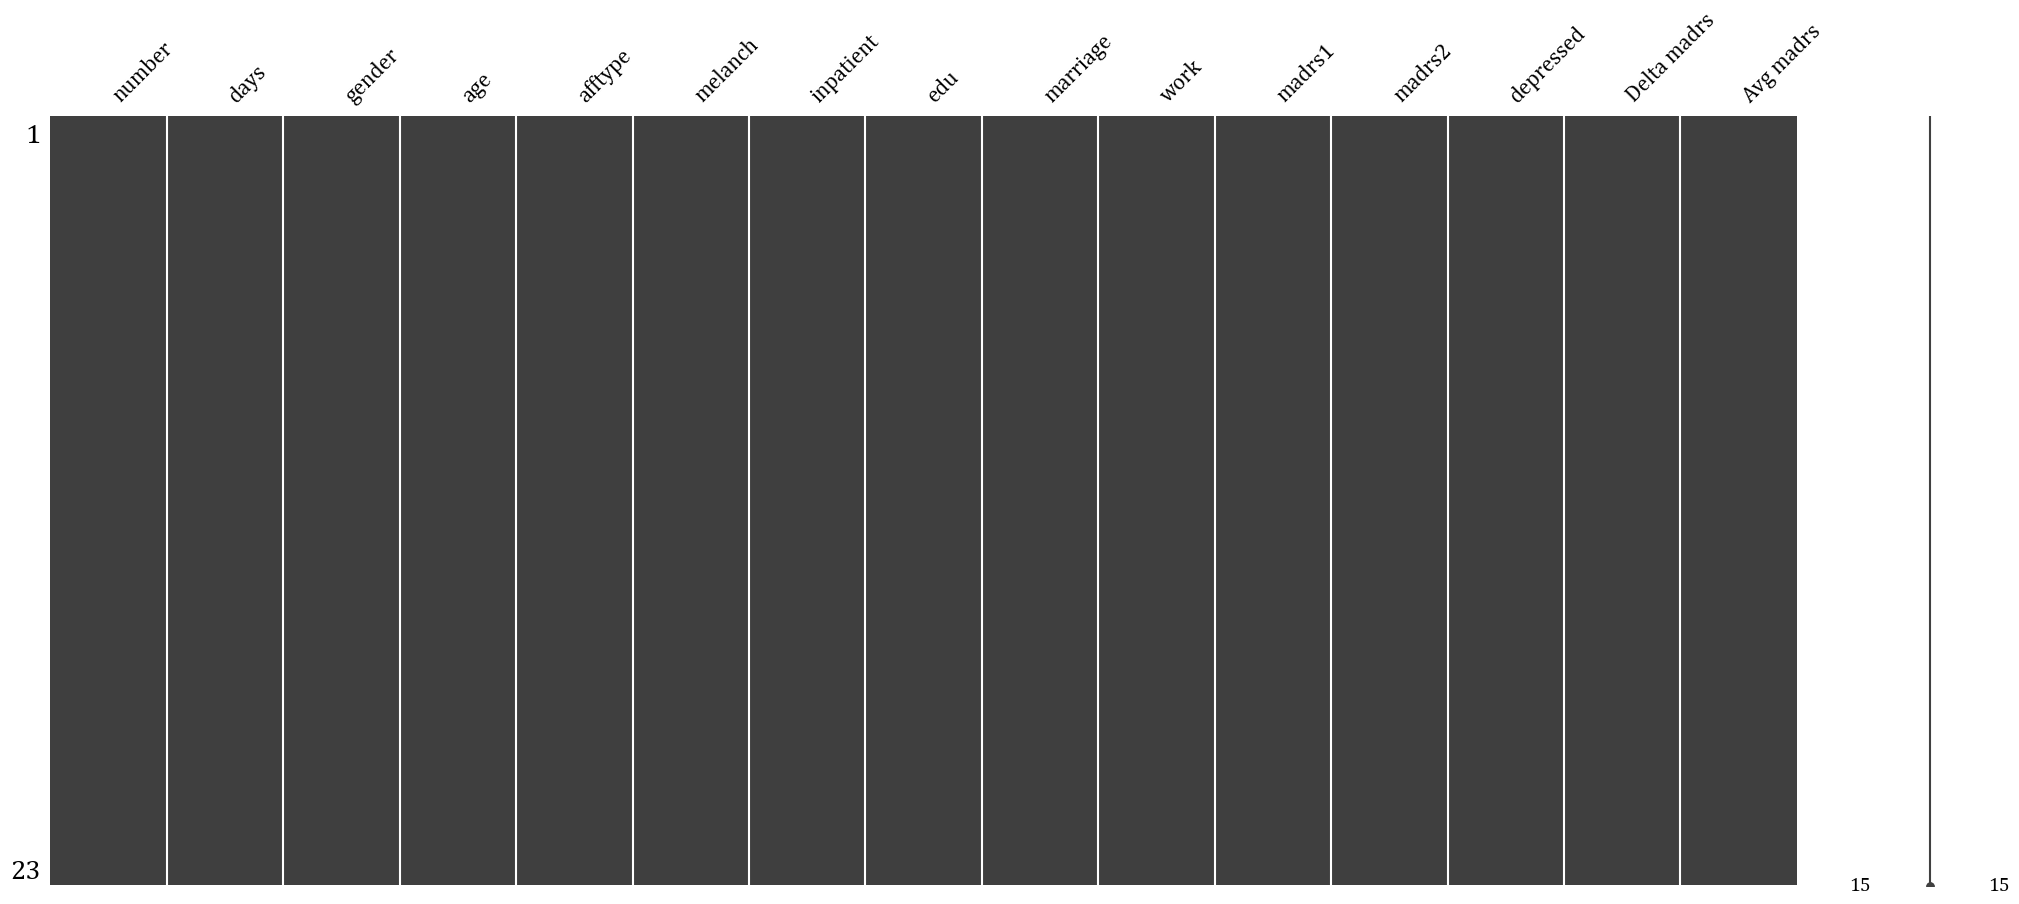
\includegraphics[scale=0.3]{images/miggingno_fin.png}
% 	\caption{Visualization of dataset post imputation.}
% 	\label{fig:missing_fin}
% \end{figure}
% 
% \noi
% \textcolor{blue}{The codes written for this section - Meta Data Imputation, can be accessed in the notebook:\\ \texttt{1\_score\_data\_preprocessing.ipynb}}

\paragraph{Actigraph Data Preprocessing}
Actigraph data from each participant was obtained. The number of samples varied for each participant as the days across which the data was collected varied. For each participant, the data was split across days and only the data where motor activity was available for entire duration (1440 minutes in a day) was used for further analysis. In order to overcome the limitations caused due to the small sample size, each day was considered as a data point for all subsequent analysis. In addition to considering only days where motor activity was available for the whole duration, data from only the days with average activity greater than a threshold activity were considered. This is explained using graphics in \autoref{fig:act_condn1}.

\begin{figure}[H]
	\centering
	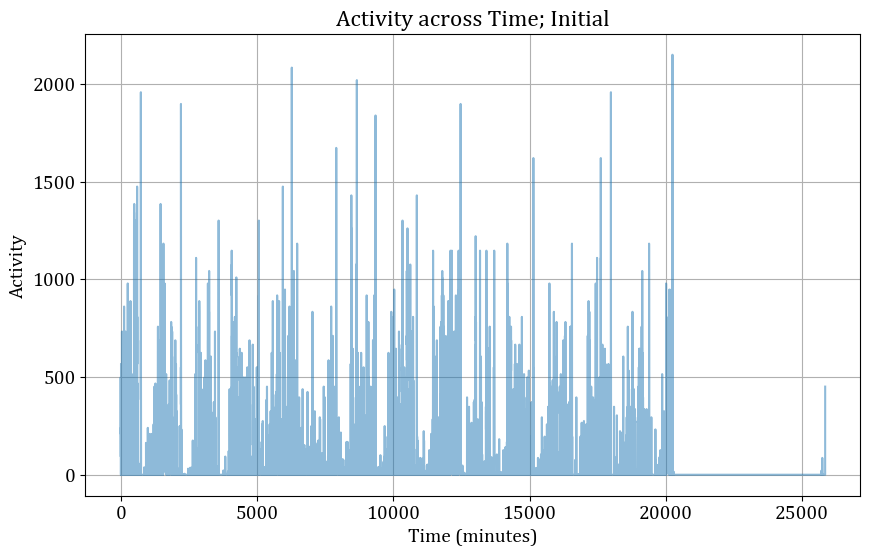
\includegraphics[scale=0.35]{images/actigraph_init.png}
	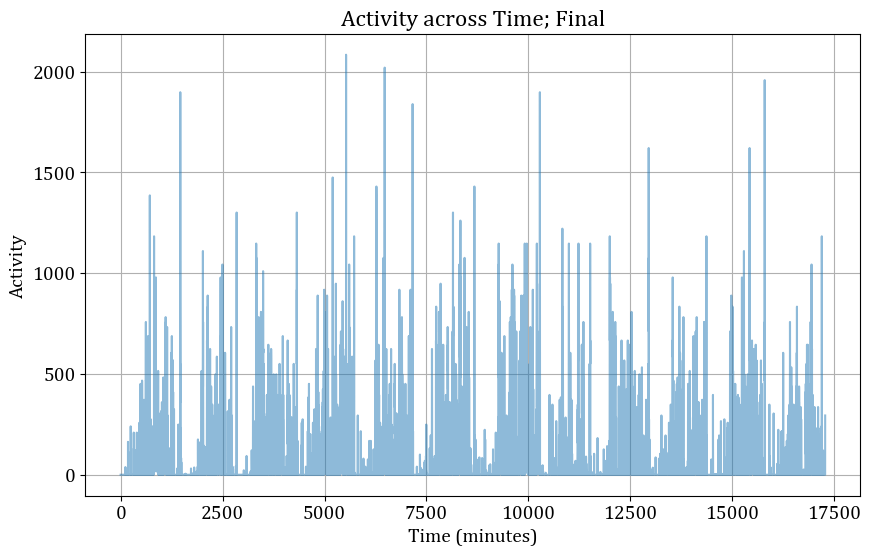
\includegraphics[scale=0.35]{images/actigraph_final.png}
	\caption{Motor Activity of Condition Participant 20. Note the extended duration of no activity towards the end in the graph on left. Final processed actigraph data on the right.}
	\label{fig:act_condn1}
\end{figure}

\noi
A consolidated dataset was obtained by stacking the data of each day for every participant across both control and condition groups. Another instance of the data was created, where the activity data was normalized for each participant, to avoid any scaling issues arising due to individual differences. 

\subsubsection{Exploratory Data Analysis}
Exploratory Data Analysis (EDA) was performed on the meta data. Pair plots and correlations were analyzed for any trends. Some observations that we can draw from the correlation plot in \autoref{fig:corr_plot} is as follows:

\begin{figure}[tb]
	\centering
	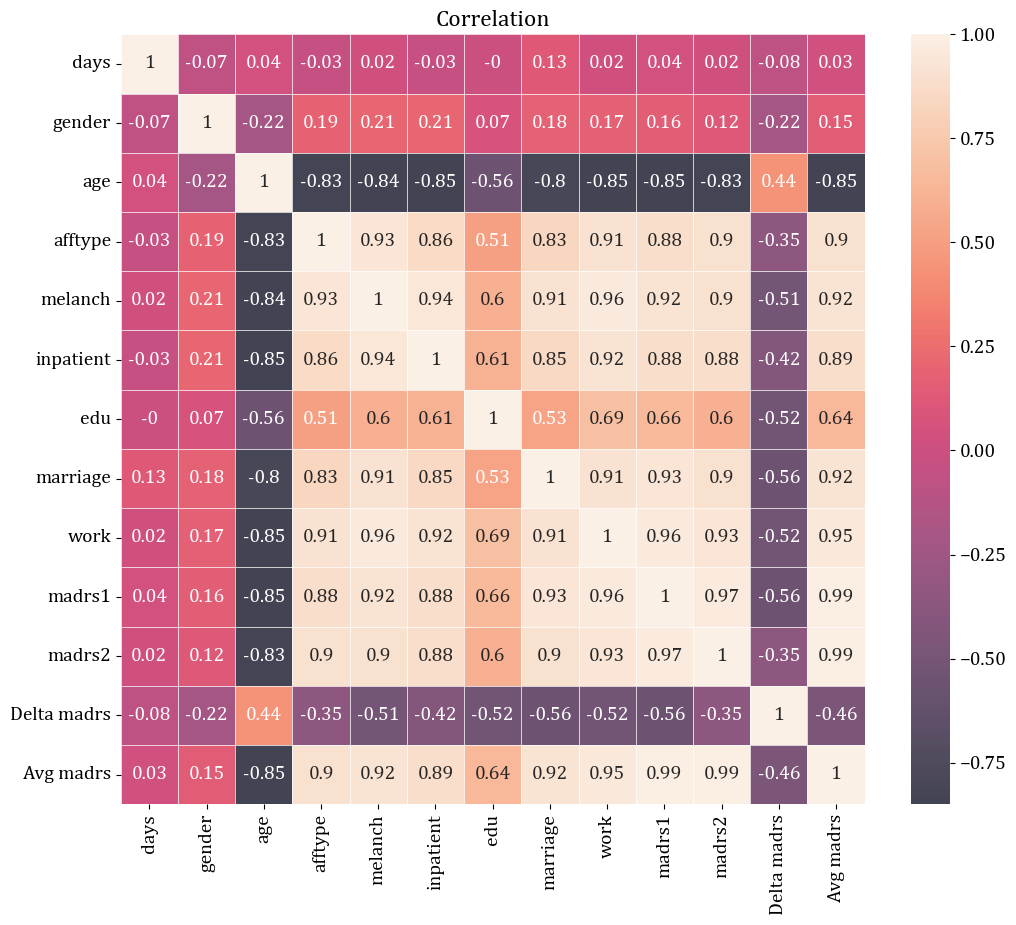
\includegraphics[scale=0.5]{images/score_corr.png}
	\caption{Correlation Analysis using entries in the meta data.}
	\label{fig:corr_plot}
\end{figure}

\begin{itemize}
	\itemsep0em
	\item \texttt{work} and (\texttt{melanch}, all \texttt{madrs} scores) are highly positively correlated. This is particularly interesting because higher values of \texttt{work} (2), indicates that the participant is unemployed/on a sick leave/receives pension. A positive correlation implies that people who are unemployed/on a sick leave/receive pension, tend to be more depressed than people who are currently working or studying.
	\item \texttt{marriage} and (\texttt{melanch}, all \texttt{madrs} scores) are highly positively correlated. A higher value of \texttt{marriage} (2) indicates that the participant is single. Hence, the positive correlation implies that single people tend to be more depressed. 
\end{itemize}

\noi
The pair plots were plotted to get a better understanding of the distribution of the values in the meta data. From the pair shown in \autoref{fig:pair_plot}, we can see that the data is lightly imbalanced in most classes. Hence, for all further analysis, the $F1$ Scoring metric will be used for model evaluation.

\begin{figure}[ht!]
	\centering
	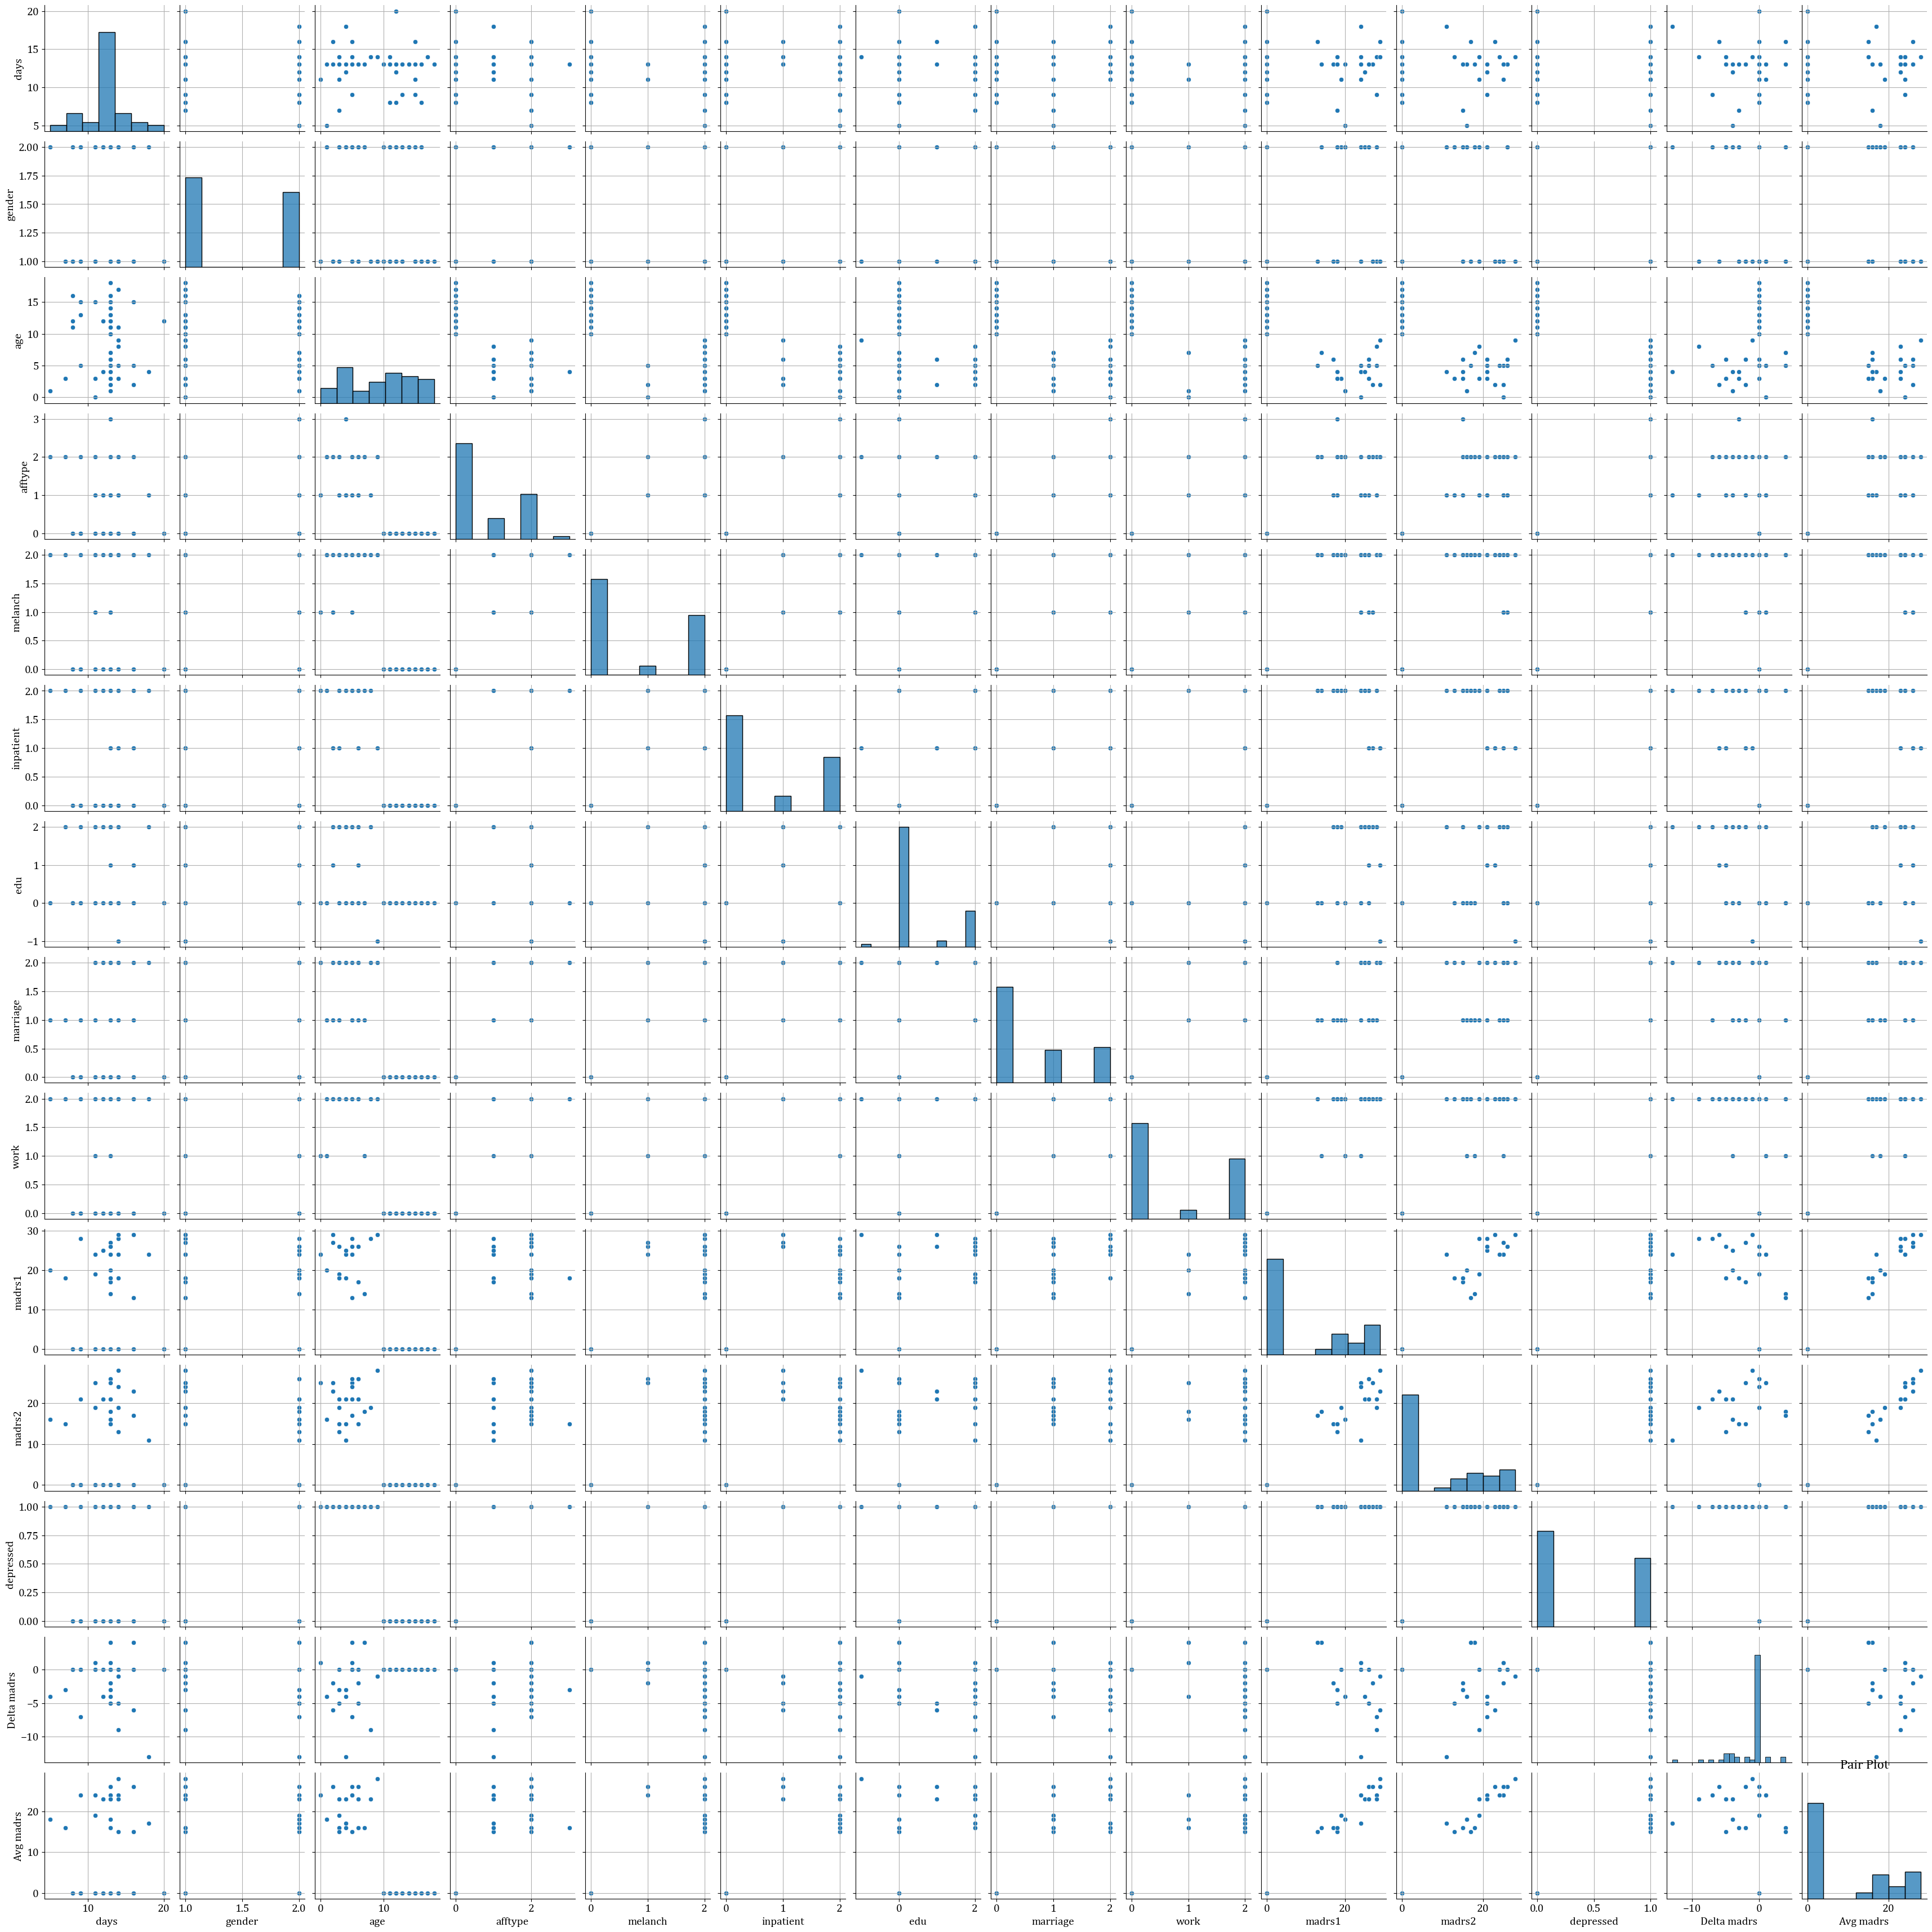
\includegraphics[scale=0.2]{images/score_pair_plot.png}
	\caption{Pair Plot of values in the meta data. Plot is made smaller for ease of representation, but is of high resolution and can be zoom in for more details.}
	\label{fig:pair_plot}
\end{figure}

\subsection{Classification Models}
In order to address all of our hypothesis, we used classification models from \texttt{sklearn}. Parameters that best explained the data was identified using Grid Search, $5$-fold cross validation and $F1$ Score as the metric. The classification models considered are as follows:
\begin{itemize}
	\itemsep0em
	\item Logistic Regression (LR)
	\item Logistic Regression (LR), with Standard Scaler
	\item Random Forest (RF)
	\item Random Forest (RF), with Standard Scaler
	\item K-Nearest Neighbors Classifier (KNN)
	\item K-Nearest Neighbors Classifier (KNN), with Standard Scaler
	\item Support Vector Machine Classifier (SVC)
	\item Support Vector Machine Classifier (SVC), with Standard Scaler
	\item Multi Layered Perceptron Classifier (MLP)
	\item Multi Layered Perceptron Classifier (MLP), with Standard Scaler
\end{itemize}

\noi
These models were trained on both unnormalized and normalized data. The parameter for each case that resulted in the best mean $F1$ score were saved and used on the validation dataset.\\

\noi
The hyperparameters considered for each model (normal and standard scaled) is as follows:
\begin{enumerate}
	\item LR: \texttt{penalty}=[\texttt{l1}, \texttt{l2}, \texttt{elasticnet}, \texttt{None}], \texttt{C}=[0.1, 0.5, 1, 10, 50], \texttt{solver}=[\texttt{liblinear},\texttt{saga}]
	\item RF: \texttt{n\_estimators}=[50, 100, 150], \texttt{min\_samples\_split}=[2, 4], \texttt{max\_features}=[\texttt{sqrt}, l\texttt{log2}]
	\item KNN: \texttt{n\_neighbors}=[3, 5, 10, 15], \texttt{weights}=[\texttt{uniform}, \texttt{distance}]
	\item SVC: \texttt{C}=[0.1, 0.5, 1, 10, 50], \texttt{kernel}=[\texttt{linear}, \texttt{poly}, \texttt{rbf}, \texttt{sigmoid}], \texttt{degree}=[3, 5, 10, 20], \\
	\texttt{decision\_function\_shape}=[\texttt{ovo}, \texttt{ovr}], \texttt{gamma}=[\texttt{auto}, \texttt{scale}]
	\item MLP: \texttt{hidden\_layer\_sizes} = [(100,), (50,), (50,10)], \texttt{activation} = [\texttt{relu}, \texttt{linear}], \texttt{alpha} = [1e-6, 1e-4, 1e-2], \texttt{learning\_rate} = [\texttt{constant}, \texttt{invscaling}, \texttt{adaptive}]
\end{enumerate}

\section{Results \& Comparisons}
The performance of the models on the training data, with the best parameter set returned is as shown below:
\begin{figure}[H]
	\centering
	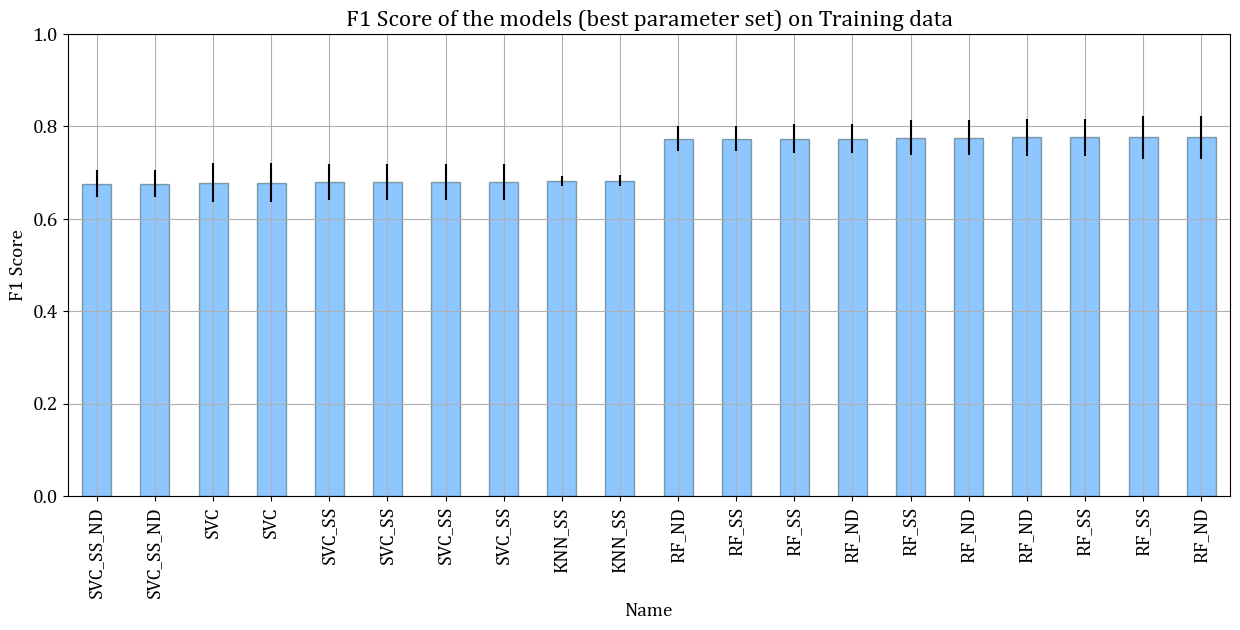
\includegraphics[scale=0.5]{images/top_20_models.png}
	\caption{F1 Scores of the top 20 Model, Parameter combinations returned by Grid Search CV.}
	\label{fig:best_models}
\end{figure}

\noi
From \autoref{fig:best_models}, the best performing models on the dataset are Random Forest Models, followed by KNN Classifiers and SVM Classifiers. For ease of representation, in all the subsequent results ``\texttt{\_ND}" indicates that the data is trained on the patient-wise normalized data; ``\texttt{\_SS}'' indicates that the whole data was standard scaled before applying the model. 

\subsection{Logistic Regression}
The top 5 model, tuned with parameters obtained using Grid Search are as follows:
\begin{table}[H]
	\centering
	\begin{tabular}{c c c c c c}
	\hline
	\hline
	\textbf{Name} & \textbf{C} & \textbf{Regularization} & \textbf{Solver} & \textbf{F1} & \textbf{Accuracy} \\ 
	\hline
	\hline
	LR\_ND & 0.5 & l1 & liblinear & 0.77 & 0.83 \\ 
	LR\_SS & 0.1 & l2 & liblinear & 0.75 & 0.78 \\ 
	LR & 50 & l2 & saga & 0.75 & 0.79 \\ 
	LR & 10 & l2 & saga & 0.75 & 0.79 \\ 
	LR & 10 & None & saga & 0.75 & 0.79 \\ 
	\hline
	\end{tabular}

	\caption{Top 5 performances of the Logistic Regression Classifier model, sorted based on validation F1 scores, for different parameter values.}
	\label{tab:lr}
\end{table}



\noi
Interpretations based on the best model parameters:
\begin{enumerate}
	\itemsep0em
	\item The best model has a relatively low \texttt{C} value. As \texttt{C} is the inverse of regularization coefficient in \texttt{sklearn}, this implies that the best model utilizes regularization to improve generalization.
	\item The regularization used by the best model is \texttt{l1} regularization. The second best model uses the \texttt{l2} regularization, but in order to achieve the same level of performance as the best model, it uses stronger regularization.
	\item The solver that gives the best F1 score is \texttt{liblinear}. It has been shown in \cite{fan2008liblinear} that \texttt{liblinear} is a very good choice for smaller datasets, in practice. 
\end{enumerate}

\subsection{Random Forest}
The top 5 model, tuned with parameters obtained using Grid Search are as follows:
\begin{table}[H]
	\centering
	\begin{tabular}{c c c c c c}
	\hline
	\hline
	\textbf{Name} & \textbf{Max Features} & \textbf{Min Samples Split} & \textbf{\# Estimators} & \textbf{F1} & \textbf{Accuracy} \\
	\hline
	\hline
	RF\_ND & sqrt & 2 & 150 & 0.89 & 0.90 \\
	RF\_ND & sqrt & 2 & 50 & 0.89 & 0.90 \\
	RF\_ND & sqrt & 2 & 100 & 0.88 & 0.90 \\
	RF\_ND & sqrt & 4 & 100 & 0.88 & 0.90 \\
	RF\_ND & sqrt & 4 & 50 & 0.87 & 0.89 \\
	\hline
	\end{tabular}

	\caption{Top 5 performances of the Random Forest Classifier model, sorted based on validation F1 scores, for different parameter values.}
	\label{tab:rf}
\end{table}



\noi
Interpretations based on the best model parameters:
\begin{enumerate}
	\itemsep0em
	\item \texttt{min\_samples\_split} of 2 gives better accuracy than of 4. As this parameter determines the minimum number of samples required to split an internal node, a smaller value would enable the model to fit the data more \textit{finely}.
	\item The best models seem to be robust to changes in the \texttt{n\_estimators} because the top 3 models all have different \texttt{n\_estimators}. The \texttt{n\_estimators} determines the number of trees in the forest, and it was interesting to note that the model fits didn't change considerably when the parameter was changed. This results is corroborated by \cite{cutler2012random} and it can be speculated that this robustness arises as a result of \textit{bagging} performed to reach a consensus.
	\item The best models have the \texttt{max\_features} parameter set to \texttt{sqrt} as opposed to \texttt{log2}. Taking into consideration the number of features in our dataset, the value returned by \texttt{sqrt} is higher than that returned by \texttt{log2}. This also indicates that when information from larger number of features (time points, in our case) are used, it results in better F1 score and accuracy.
\end{enumerate}


\subsection{K-Nearest Neighbors}
The top 5 model, tuned with parameters obtained using Grid Search are as follows:
\begin{table}[H]
	\centering
	\begin{tabular}{c c c c c}
	\hline
	\hline
	\textbf{Name} & \textbf{Neighbors} & \textbf{Weights} & \textbf{F1} & \textbf{Accuracy} \\ 
	\hline
	\hline
	KNN &  10 & distance & 0.84 & 0.81 \\ 
	KNN\_SS & 10 & distance & 0.84 & 0.81 \\ 
	KNN &  15 & distance & 0.82 & 0.79 \\ 
	KNN\_ND &  3 & distance & 0.81 & 0.78 \\ 
	KNN\_SS & 5 & distance & 0.81 & 0.79 \\ 
	\hline
	\end{tabular}

	\caption{Top 5 performances of the KNN Classifier model, sorted based on validation F1 scores, for different parameter values.}
	\label{tab:knn}
\end{table}



\noi
Interpretations based on the best model parameters:
\begin{enumerate}
	\itemsep0em
	\item The best models have the \texttt{n\_neighbors} parameter value of 10. When this is increased or decreased, there is a small dip in the F1 score and accuracy. This implies that only the closest 10 neighbors are relevant to the data point of interest, thereby giving us an intuition about the distribution of the data points in our dataset.
	\item All the top 5 models used the \texttt{weights} parameter of \texttt{distance} as opposed to \texttt{uniform}. This highlights that the relative distance between the data points is more informative than when compared to using a uniform weight distribution, when making a prediction.
\end{enumerate}

\subsection{Support Vector Machines}
The top 5 model, tuned with parameters obtained using Grid Search are as follows:
\begin{table}[H]
	\centering
	\begin{tabular}{c c c c c c c c}
	\hline
	\hline
	\textbf{Name} & \textbf{C}& \textbf{Decision Function} & \textbf{Degree} & \textbf{$\gamma$} & \textbf{Kernel} & \textbf{F1} & \textbf{Accuracy} \\
	\hline
	\hline
	SVC\_SS & 10 & ovo & 3 & auto & poly & 0.84 & 0.85\\
	SVC\_SS & 10 & ovr & 3 & auto & poly & 0.84 & 0.85\\
	SVC & 10 & ovo & 3 & scale & poly & 0.82 & 0.83\\
	SVC\_SS & 10 & ovo & 3 & scale & poly & 0.82 & 0.83\\
	SVC\_SS & 10 & ovr & 3 & scale & poly & 0.82 & 0.83\\
	\hline
	\end{tabular}

	\caption{Top 5 performances of the SVM Classifier model, sorted based on validation F1 scores, for different parameter values.}
	\label{tab:svc}
\end{table}



\noi
Interpretations based on the best model parameters:
\begin{enumerate}
	\itemsep0em
	\item The value of 10 for the \texttt{C}, inverse regularization parameter seemed to give raise to best predictions. The next best values of \texttt{C} reported by grid search are 50, followed by 0.5 and 0.1. This implies that the sweet spot for the regularization parameter is 10, and higher values would result in higher variance and lower values would result in higher bias.
	\item All the 5 top models used a \texttt{degree} of 3. This in conjunction to the \texttt{kernel} being set to \texttt{poly} gives us an intuition that the best mapping from the actigraph space to the classification is a non-linear, polynomial mapping of degree 3.
	\item The best models were robust to the \texttt{decision\_function\_shape} used. This is intuitive as all the models were trained on a binary-class classification task.
	\item The parameter \texttt{gamma} is the inverse of the radius of influence of a single training sample. When large values of \texttt{gamma} is used, the radius of influence becomes small and results in over-fitting. Similarly, when small values of \texttt{gamma} is used, the radius of influence becomes large and results in under-fitting. The value of \texttt{auto} as opposed to \texttt{scale} best fits the dataset and implies that it is not essential to make \texttt{gamma} dependent on the variance of the dataset.
\end{enumerate}

\subsection{Multi-layered Perceptrons}
The top 5 model, tuned with parameters obtained using Grid Search are as follows:
\begin{table}[H]
	\centering
	\begin{tabular}{c c c c c c c}
	\hline
	\hline
	\textbf{Name} & \textbf{Activation} & \textbf{$\alpha$} & \textbf{\# Nodes} & \textbf{LR Scheduler} & \textbf{F1} & \textbf{Accuracy} \\ 
	\hline
	\hline
	MLP\_ND & relu & 0.0001 & (50, 10) & invscaling & 0.81 & 0.84 \\ 
	MLP\_SS\_ND & relu & 0.0001 & (50, 10) & adaptive & 0.81 & 0.84 \\ 
	MLP\_SS\_ND & relu & 0.0001 & (50, 10) & invscaling & 0.81 & 0.84 \\ 
	MLP\_SS\_ND & relu & 0.0001 & (50, 10) & constant & 0.81 & 0.84 \\ 
	MLP\_ND & relu & 0.0001 & (50, 10) & adaptive & 0.81 & 0.84 \\  
	\hline
	\end{tabular}

	\caption{Top 5 performances of the MLP Classifier model, sorted based on validation F1 scores, for different parameter values.}
	\label{tab:mlp}
\end{table}



\noi
Interpretations based on the best model parameters:
\begin{enumerate}
	\itemsep0em
	\item The best models all utilized the \texttt{relu} activation function as opposed to \texttt{tanh}. This in in conjunction with the recent trends in deep learning \cite{fukushima1980neocognitron}, \cite{nair2010rectified}, \cite{agarap2018deep}.
	\item Lower value of \texttt{alpha}, coefficient of regularization, has been opted by all the best models.
	\item All the best models use a \texttt{hidden\_layer\_sizes} of (50, 10). This shows that the model with two layers performs better than when compared to models that have a single hidden layer. This potentially ties to the models' ability to extract more information from the dataset in the presence of additional layers.
	\item The models seem to be robust to the choice of \texttt{learning\_rate} scheduler used. However, from the results, we see that \texttt{invscaling} and \texttt{adaptive} are better represented than \texttt{constant}, indicating that dynamic adjustments to learning rates is more advantageous than static learning rates.
\end{enumerate}

\subsection{Model Selection}
The top 15 models and parameter combinations presented in \autoref{fig:best_models} were subsequently used to address all the proposed hypothesis. Across all models, when PCA was applied on the data prior to model fitting, the performance dropped. Hence, PCA based dimensionality reduction was not used in all subsequent analysis.


\section{Results Visualization}
\subsection{Hypothesis 1}
The model performance of Random Forest Classifiers and Logistic Regression Classifiers was obtained. As observed in the previous section, the best model performance are as follows:
\begin{itemize}
	\itemsep0em
	\item Logistic Regression: F1 Score: 0.77; Accuracy: 0.83
	\item Random Forest: F1 Score: 0.89; Accuracy: 0.90
\end{itemize}

\begin{figure}[H]
	\centering
	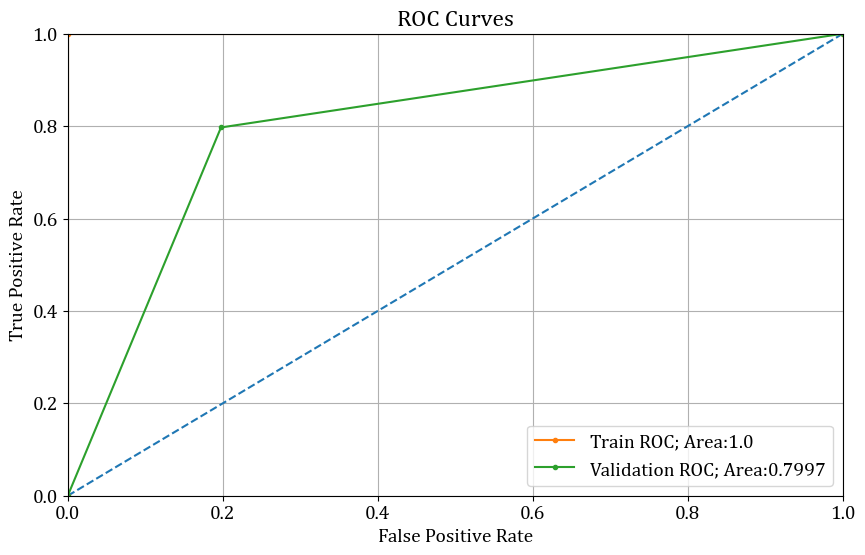
\includegraphics[scale=0.26]{images/H1_roc_corve.png}
	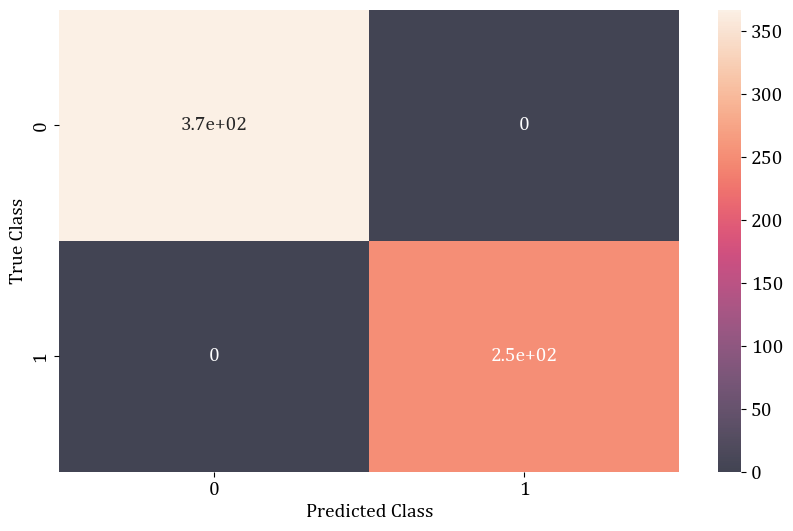
\includegraphics[scale=0.26]{images/H1_confusion_matrix.png}
	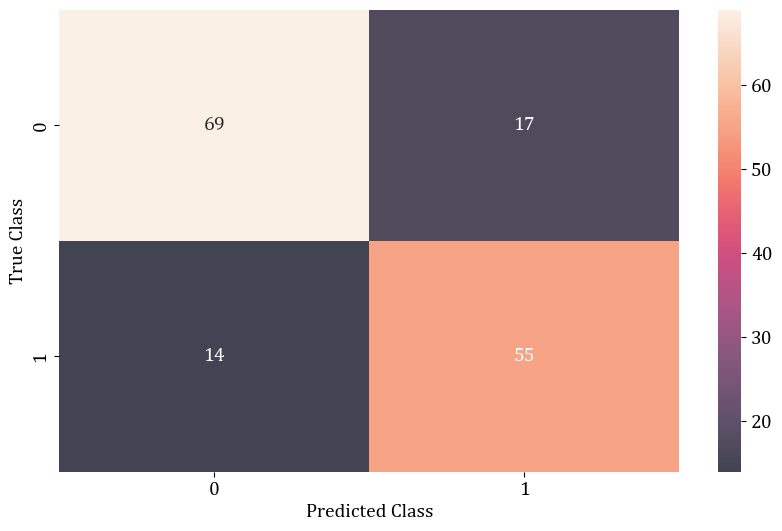
\includegraphics[scale=0.26]{images/H1_confusion_matrix_val_test.png}
	\caption{ROC Curve and Confusion Matrix (train, validation) for the best model; Hypothesis 1}
	\label{fig:H1_roc_conf}
\end{figure}

\noi
As we can see above, the best Random Forest model provides a really good fit to the dataset and is able to perform better, both in terms of accuracy and F1 score, than when compared to Logistic Regression.

\subsection{Hypothesis 2}
Since the data is arranged in a day-wise format across all participants, the age and gender information for all participants was tiled and stacked with the actigraph dataset. This dataset comprising actigraph information, age and gender data was used for analysis in this section.\\

\noi
When the age and gender data was included, both the F1 score and accuracy increased slightly. The best model results are: F1 Score: 0.925926 and Accuracy: 0.935484. The ROC Curve and Confusion Matrix of the best model is shown in \autoref{fig:H2_roc_conf}. From the confusion matrix we can see that the model is able to correct some of the wrongly classified data points when the age and gender information is added.

\begin{figure}[H]
	\centering
	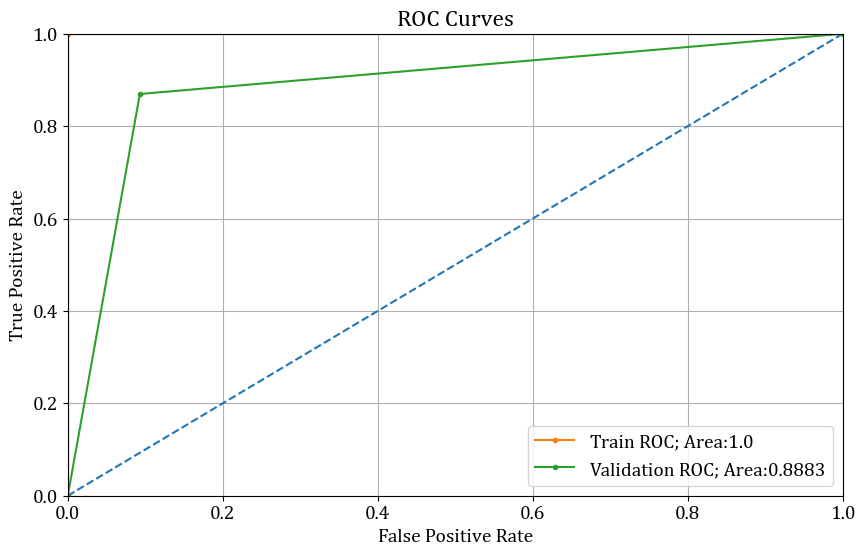
\includegraphics[scale=0.26]{images/H2_roc_corve.png}
	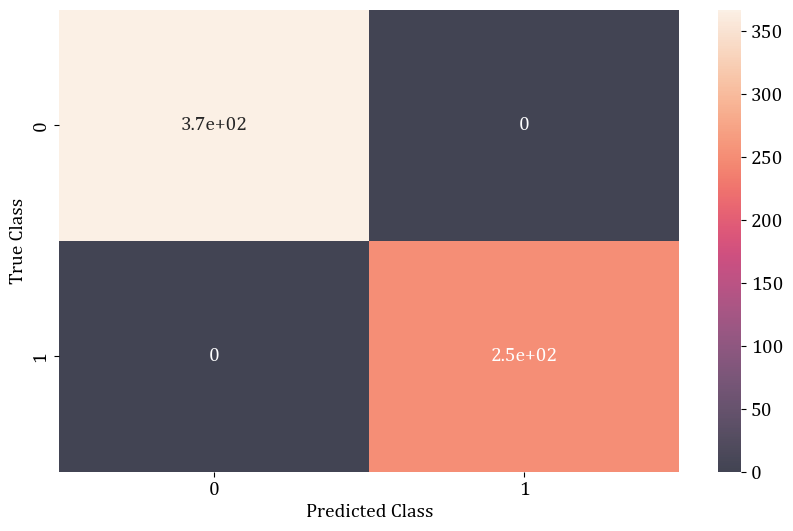
\includegraphics[scale=0.26]{images/H2_confusion_matrix.png}
	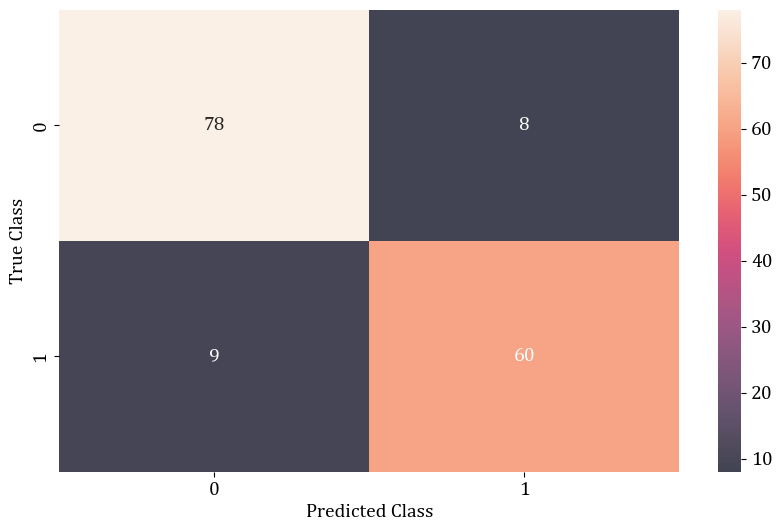
\includegraphics[scale=0.26]{images/H2_confusion_matrix_val_test.png}
	\caption{ROC Curve and Confusion Matrix (train, validation) for the best model; Hypothesis 2}
	\label{fig:H2_roc_conf}
\end{figure}


\subsection{Hypothesis 3}
The same dataset generated for the last hypothesis was used here. The best model results are: F1 Score: 0.925926 and Accuracy: 0.935484. The ROC Curve and Confusion Matrix of the best model is shown in \autoref{fig:H2_roc_conf}. The accuracies and F1 scores for males and females obtained from the model that best fit the dataset is as follows:
\begin{itemize}
	\itemsep0em
	\item Male: Accuracy: 0.953846; F1 Score: 0.958904
	\item Female: Accuracy: 0.831325; F1: 0.758621
\end{itemize}

\subsection{Hypothesis 4}
A similar approach as in Hypothesis 2 was taken to generate a dataset that had information about the level of depression in a patient. Both the MADRS Scores 1 and 2 were included in the dataset. 

\noi
The accuracies and F1 scores for mild and severe depression obtained from the model that best fit the dataset (same model as the previous subsection) is as follows:
\begin{itemize}
	\itemsep0em
	\item Mild Depression: Accuracy: 0.972727; F1: 0.938776
	\item Severe Depression: Accuracy: 0.822222; F1: 0.902439
\end{itemize}

\begin{figure}[H]
	\centering
	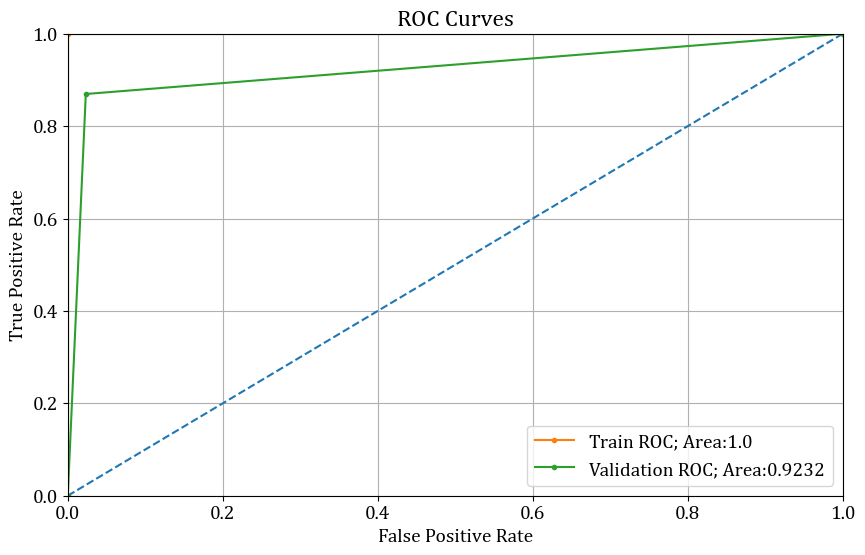
\includegraphics[scale=0.26]{images/H4_roc_corve.png}
	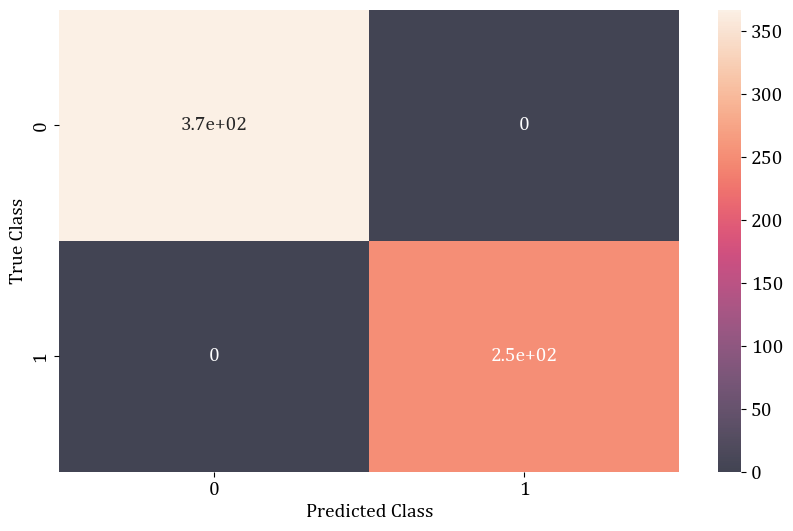
\includegraphics[scale=0.26]{images/H4_confusion_matrix.png}
	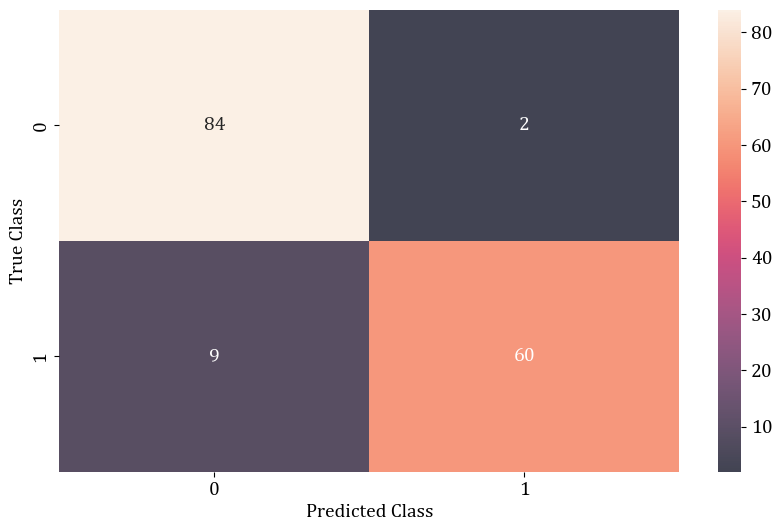
\includegraphics[scale=0.26]{images/H4_confusion_matrix_val_test.png}
	\caption{ROC Curve and Confusion Matrix (train, validation) for RF model.}
	\label{fig:H4_roc_conf}
\end{figure}

\section{Discussion}
This study aimed to determine which classification model could most accurately predict depression based on motor activity recorded from an Actigraph wearable wristband. Our study used motor Actigraph data from \cite{garcia2018depresjon}. \\

\noi
In our analysis, we used 5 different classes of models, namely Logistic Regression, Random Forest, K-Nearest Neighbors Classifier, Support Vector Machine Classifier, and Multi-Layer Perceptron Classifier. We sought to determine which model parameters would enable the best predictor of depression from motor activity. We utilized a dataset comprising 773 data points, with 340 belonging to the depressed condition and the remaining samples serving as controls. \\

\noi
As the number of features (activity per minute) in our data was 1440, representing a high-dimensional data space, we attempted to use Principal Component Analysis (PCA) to reduce the dimensionality of our dataset and identify the most relevant features. However, we found that this approach did not significantly improve our model's performance and did not use PCA based dimensionality for our subsequent analyses. This indicates that specific motor activity features are critical for distinguishing between individuals with depression and those without. Jointly considering the \texttt{kernel} results from \texttt{SVC} and the results from \texttt{PCA}, we can see that the mapping between the actigraph space and the output space is non-linear. Which could also explain why PCA, a linear dimensionality reduction technique did not result in better classification accuracies.\\

\noi
The best parameters for each model were identified using grid search, combined with a 5-fold cross validation on the training sample. The models that best differentiated between the control and condition groups are the Random Forest models, Support Vector Machine Classifier models and K-Nearest Neighbors Classifier models, in the same order. \\

\noi
We found that the random forest model could accurately classify the samples' condition status with a high F1 score and accuracy. The superior performance of the random forest model can be attributed to its ability to handle high-dimensional data by constructing a large number of decision trees and the use of bagging to combine their results to make the final classification decision. This approach is advantageous when dealing with complex data structures where traditional regression models may not be sufficient. Our findings support the use of RF models as a powerful tool for classification tasks in mental health research when the dataset is small and has a large number of features. \\

\noi
We also developed a logistic regression model to predict depression based on motor activity. We investigated the impact of regularization and solver algorithms on the model's predictive performance. Our findings indicate that logistic regression was robust to both the coefficient and type of regularization, i.e., \texttt{L1} and \texttt{L2} regularization, but \texttt{L2} utilizes a larger regularization coefficient than \texttt{L1} to achieve the same level of performance. We compared two solver algorithms for logistic regression, \texttt{liblinear} and \texttt{saga}. Our results indicate that on our small dataset \texttt{liblinear} performs better than \texttt{saga}. However, when the data was not normalized or standard scaling was not used, \texttt{saga} performed better than \texttt{liblinear}. This could be attributed to \texttt{liblinear}'s tendency to converge at a non-stationary point, leading to suboptimal model performance. Our findings suggest that while logistic regression is a robust model for predicting depression based on motor activity, it is outperformed by the RF model.\\

\noi
We further investigated the impact of adding age and sex data to our predictive models for depression classification based on motor activity. Our findings indicate that including age and sex data improved the model's classification performance. Additionally, we observed that our models had higher accuracies and F1 scores for males than females. This suggests that there may be gender-based differences in the impact of motor activity on depression. We also investigated the model performances in accurately predicting mild and severe depression. We found that when control samples were included, the accuracy and F1 score of mild depression cases were higher than severe depression cases. This suggests that including control samples may provide additional information that could aid in better differentiating between mild and severe depression cases based on motor activity.\\

\noi
While our study provides valuable insights into using RF models for depression classification, several limitations must be acknowledged. Our dataset was relatively small, and future studies with larger sample sizes are required to confirm our findings. Furthermore, there are limitations to using motor activity as the sole feature for depression classification. Our dataset does not account for the individual variability in movement and fails to account for other symptoms of depression, such as one's mood or cognitive state. Additionally, we did not explore the potential impact of confounding variables on our results, such as medication use or comorbid conditions. Future studies should address these limitations and further refine our understanding of the role of motor activity in depression.



\break
\bibliographystyle{apalike}
\bibliography{references}

\end{document}